\newcount\draft\draft=1 % set to 0 for submission or publication
\documentclass[sigplan,review,anonymous]{acmart}
\setcopyright{none}
%
\usepackage{tikz}
\usetikzlibrary{snakes}
\usepackage[norelsize]{algorithm2e}
\usepackage{xxx}
\usepackage{fncylab}
\usepackage{subcaption}
%
\usepackage{graphicx}
% Used for displaying a sample figure. If possible, figure files should
% be included in EPS format.
%
% If you use the hyperref package, please uncomment the following line
% to display URLs in blue roman font according to Springer's eBook style:
% \renewcommand\UrlFont{\color{blue}\rmfamily}
\AtBeginDocument{%
  \providecommand\BibTeX{{%
    \normalfont B\kern-0.5em{\scshape i\kern-0.25em b}\kern-0.8em\TeX}}}

\labelformat{algocf}{algorithm\,(#1)}

\begin{document}
\settopmatter{printacmref=false}
\title{Online Verification of Commutativity}
%
%\titlerunning{Abbreviated paper title}
% If the paper title is too long for the running head, you can set
% an abbreviated paper title here
%
\author{First Author}
\email{email}
\author{Second Author}
\authornotemark[1]
\email{email 2}
\affiliation{%
  \institution{Cornell University}
  \streetaddress{address}
  \city{Ithaca}
  \state{New York}
  \postcode{14850}
}

\author{Third Author}
\email{email 3}

\begin{abstract}
Systems of transformations arise in many programming systems, such as in type graphs of implicit type conversion functions.
It is important to ensure that these diagrams commute: that any composing path of transformations from the same source to the same destination yields the same result.
However, a straightforward approach to verifying commutativity must contend with cycles, and even so it runs in exponential time.
Previous work has shown how to verify commutativity in the special case of acyclic diagrams in $O(|V|^4|E|^2)$ time,
% I think this is clear enough (at least for the abstract). --AS
% where V is the set of vertices in the diagram, and E, the set of edges.
but this is a \emph{batch} algorithm: the entire diagram must be known ahead of time.
We present an \emph{online} algorithm that efficiently verifies that a commutative diagram remains commutative when adding a new edge.
The new incremental algorithm runs in $O(|V|^2(|E| + |V|))$ time.
For the case when checking the equality of paths is expensive, we also present an optimization that runs in $O(|V|^4)$ time but reduces to the minimum possible number of equality checks.
We implement the algorithms and compare them to batch baselines, and we demonstrate their practical application in the compiler of a domain-specific language for geometry types.
To study the algorithms' scalability to large diagrams, we apply them to discover discrepancies in currency conversion graphs.
\end{abstract}

\maketitle

\section{Introduction}
Many systems can be understood as diagrams: graphs where nodes represent domains and edges represent directed transformation functions between nodes.
A type system with coercions, for example, corresponds to a graph whose nodes are types and whose edges are coercions.
Figure~\ref{fig:typeExample} illustrates an example in a simple language with units-of-measure types.
\xxx[as]{Refer here to some citations of real type systems for units of measure.}
In such a system, an important correctness criterion is that the diagram \emph{commutes:} when traversing the graph from any start node to any end node, applying every transformation along the path to any input value, the result is the same output value \emph{independent of the path chosen between the two nodes}.
With our type coercion example, it is a problem if casting to a supposedly equivalent type as an intermediate step resulted in a different answer than a direct cast.
\xxx[as]{Next, let's make the example specific: say that the expression ``(wugs) a'', for example, can produce value X or value Y, depending on whether the compiler uses path A or path B to do the conversion.}

\begin{figure}[]
    \centering
    \begin{subfigure}{0.4\textwidth}
        \begin{verbatim}
            var a : meters = 1;
            var b : miles = (miles) a;
            var c : feet = (feet) a;
            define wugs:
                1 miles = 10000 wugs;
                1 foot = 10 wugs;
            var d : wugs = (wugs) a;
        \end{verbatim}
        \caption{A sample program with user defined type conversion.}
    \end{subfigure}

    \begin{subfigure}{0.4\textwidth}
        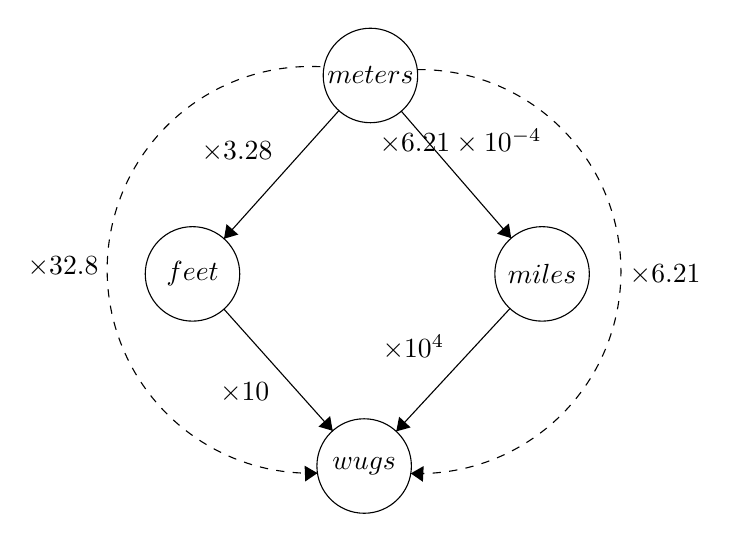
\begin{tikzpicture}[scale=0.2]
            \tikzstyle{every node}+=[inner sep=0pt]
            \draw [black] (32.8,-8.8) circle (3);
            \draw (32.8,-8.8) node {$meters$};
            \draw [black] (21.5,-21.4) circle (3);
            \draw (21.5,-21.4) node {$feet$};
            \draw [black] (43.7,-21.4) circle (3);
            \draw (43.7,-21.4) node {$miles$};
            \draw [black] (32.4,-33.6) circle (3);
            \draw (32.4,-33.6) node {$wugs$};
            \draw [black] (30.8,-11.03) -- (23.5,-19.17);
            \fill [black] (23.5,-19.17) -- (24.41,-18.9) -- (23.66,-18.24);
            \draw (26.61,-13.64) node [left] {$\times 3.28$};
            \draw [black] (34.76,-11.07) -- (41.74,-19.13);
            \fill [black] (41.74,-19.13) -- (41.59,-18.2) -- (40.84,-18.85);
            \draw (43.7,-13) node [left] {$\times 6.21 \times 10^{-4}$};
            \draw [black] (23.5,-23.64) -- (30.4,-31.36);
            \fill [black] (30.4,-31.36) -- (30.24,-30.43) -- (29.5,-31.1);
            \draw (26.41,-28.96) node [left] {$\times 10$};
            \draw [black] (41.66,-23.6) -- (34.44,-31.4);
            \fill [black] (34.44,-31.4) -- (35.35,-31.15) -- (34.62,-30.47);
            \draw (37.52,-26.04) node [left] {$\times 10^4$};
            \draw [dashed] (29.441,-34.049) arc (-88.02206:-273.82603:12.915);
            \fill [black] (29.44,-34.05) -- (28.62,-33.58) -- (28.66,-34.58);
            \draw (15.56,-20.93) node [left] {$\times 32.8$};
            \draw [dashed] (35.77,-8.425) arc (90.49177:-92.33986:12.828);
            \fill [black] (35.36,-34.07) -- (36.13,-34.6) -- (36.18,-33.6);
            \draw (49.23,-21.46) node [right] {$\times 6.21$};
            \end{tikzpicture}
        \caption{Diagram for the type conversions in the program}
    \end{subfigure}

    \caption{In this sample program, the user implicitly defines two ways to cast variable a from meters to the new unit wugs.
    The definitions are different, and a compiler performing implicit conversion would not know which to choose.}
    \label{fig:typeExample}
\end{figure}

This paper is about efficiently checking diagrams that arise in real systems for commutativity.
We assume a simple equivalence checker for individual transformation functions: in our type system example, for instance, it is possible to check transformation equivalence by comparing the conversion factors.
Our aim is to analyze the graph of transformations and minimize the number of times we need to perform an equivalence check.
Since diagrams may change over time in real systems, as new conversions are added, and verifying the entire system from scratch may be computationally expensive, we want an online method that only checks the impact of new edges.
In Figure~\ref{fig:typeExample}, for example, a run-time system can catch the point where the programmer adds a bad conversion definition by verifying each new conversion edge as it is created.

Efficient commutativity checking is not trivial.
\xxx[as]{Let's flip these next two thoughts, because the first thing you have to deal with is resolving cycles---then you can worry about an efficient algorithm for acyclic graphs.}
Na\"{i}vely checking if all path pairs that begin and end at the same node in a given diagram commute could require a number of function equality checks that grow as factorial in the number of nodes, because a path consists of an ordering of nodes.
Further, the presence of cycles implies a potentially infinite number of paths.
Previous work ~\cite{commutative} has identified an $O(|E|^2|V|^4)$ algorithm to verify that a complete acyclic diagram commutes; however, it addresses neither online addition nor cyclic diagrams.

\xxx[as]{Let's stick to present tense, even if it sounds a little weird. And we can state up front what the paper accomplishes. Something like this: ``This paper presents an algorithm for online checking of diagram commutativity and applies it to verifying systems of value conversions. We identify two key insights:''}
In the course of efficiently verifying commutativity over online addition, we identified two key insights.
The first was that in a commutative diagram, when a new edge is to be added, at most one path needs to be checked against \xxx[as]{can we rephrase this passive voice, which makes the sentence somewhat tricky to process?} for a given source and sink pair.
Because the diagram commutes, all the paths between a given source and sink are equal and a representative to check against can arbitrarily be chosen.
It lead to an $O(|V|^2(|E|+|V|))$ algorithm to verify a diagram remains commutative over the course of online addition, assuming an oracle to check the equality of functions.
The algorithm makes an asymptotically optimal number of calls to the oracle.

\xxx[as]{This paragraph is a little confusing to me. First, what is ``informativeness''? Maybe we can be a little more specific. Second, I thought the previous paragraph said we already had an optimal number of calls to the oracle, but the second half of this paragraphs says that we need an even more expensive algorithm to obtain that minimum.}
The second insight was that there is a single rule that places a partial, transitive ordering on the informativeness of paths.
It allowed for the creation of a greedy, $O(|V|^4)$ optimization step that results in the number of calls to the oracle being minimal.
The optimization is very useful when the equality checking oracle is expensive.

We evaluate our algorithms against random graphs and use them in two case studies.
\xxx[as]{Let's avoid passive voice in these next two sentences by saying ``we use the algorithm to do this'' instead of ``the algorithm is used to do this.''}
First, our algorithm is used in the domain specific geometry type language \textit{Gator} ~\cite{gator} to ensure that user defined transformations between spaces stay consistent.
Second, our algorithm is used to identify inefficiencies in a currency conversion graph.

We empirically compare our solution to three baseline implementations: a na\"{i}ve checking of all path pairs with only special handling for cycles, a check for all path pairs that involve the new edge, and an algorithm suggested by previous work to solve the batch version of the problem for acyclic diagrams.
Our proposed algorithms run orders of magnitude faster than the baselines.

\section{Formal Problem Setup and Terminology}

We start by formalizing the notion of a diagram, drawing terminology from the previous acyclic work by Murota~\cite{commutative}.

\paragraph{Notation.}

We start with a directed graph $G=(V,E)$, where $V$ corresponds to sets of elements and edges $(u, v)$ in $E$ correspond to functions that maps elements of $u$ to elements in $v$.
All these functions form a semigroup $F$, where multiplication is function composition.
A semigroup consists of a set and an associative binary operation, which we use to capture function composition.
%
The correspondence between edges and functions is stored as a mapping $f:E\rightarrow F$, where $f$ maps each edge to the function it represents.

A path is a sequence of edges. The edge-to-function mapping $f$ can be naturally extended to paths: if path $p=e_1\circ e_2 \circ \cdots \circ e_n$ then $f(p)=f(e_1) \circ f(e_2) \circ \cdots \circ f(e_n)$.
%
We write $\partial(p)^{+}$ for $p$'s start node, $\partial(p)^{-}$ for its end node, and $\partial(p)$ to denote the pair
$(\partial(p)^{+}, \partial(p)^{-})$.
\xxx[as]{Simplified this explanation; I hope it's OK.}

A pair of paths $p$ and $q$ is called \textit{parallel} iff their terminal nodes are the same, i.e., $\partial(p)=\partial(q)$.
$\partial$, $\partial^{+}$ and $\partial^{-}$ are extended to apply to parallel pairs.
\xxx[as]{Let's use a name other than $p$, which we have already used for paths, for pairs. (Or use something else for paths above.) Also, since we just used $p$ and $q$ for two paths, maybe that would be better than $p_1$ and $p_2$.}
For parallel pair $p$ = ($p_1$, $p_2$), $\partial(p)=\partial(p_1)=\partial(p_2)=(\partial(p)^{+}, \partial(p)^{-})$.

Let $R_{all}$ be the set of all parallel pairs of paths in a given diagram.
The diagram commutes iff
$\forall (p,q)\in R_{all}$,
$f(p)=f(q)$; that is, the composition of maps along any path connecting any pair $u$ to $v$ is independent of path choice.

\paragraph{Problems.}

The \textsc{Online addition problem}, given a commuting diagram and a new edge, returns whether the diagram commutes.
Checking function equality is a domain specific, potentially hard problem, dependent on the nature of the graph.
For our case study in graphics programming (see Section~\ref{sec:gator}), edges are matrices and nodes are vector spaces, so function composition uses matrix multiplication and equivalence checking simply compares matrix values.
We therefore assume some oracle for checking transformation function equivalence that will vary by domain.
%
We therefore reduce the \textsc{Online addition problem} to the \textsc{Verification set problem}.
\xxx[as]{Although it's not technically a ``reduction,'' is it? Maybe better to say that the latter is what we solve, and we assume an oracle that uses those results to solve the former.}
The latter, when given a diagram and a new edge, returns the set of parallel pairs of paths, such that if and only if the members in each pair are equal, then the new graph must commute.
\xxx[as]{Let's be precise around the ``equal'' terminology in the previous and next sentences. It's not that the pairs are equal---it's that we check function equivalence for the pairs' corresponding functions.}
The output to the \textsc{Online addition problem} can then be obtained as whether equality checking for all pairs succeeds.

The algorithms in the rest of the paper assume that the function equivalence oracle is reflexive, symmetric, and transitive.
\xxx[as]{The following is a little tricky to understand here... maybe this is best left to the currency section?}
For example, the oracle for currency graph (Section~\ref{sec:currency}) only approximately preserves transitivity because of floating point error magnification, so while the algorithm catches mistakes, it does not guarantee that the diagram commutes.

\section{Baseline Algorithms}

To examine the efficacy of our proposed solution to the \textsc{Verification set problem}, we compare it to some potential alternatives.
Specifically, we examine a na\"{i}ve factorial algorithm, a slightly less na\"{i}ve factorial algorithm which we identify to be a two-flip tolerant path search, and Murota's historical batch solution~\cite{commutative}.

\subsection{Na\"{i}ve Baseline}

We start with the set of all parallel pairs in the diagram (with the new edge added in), and pare it down to be finite by handling cycles.
Then, using a procedure like Johnson's algorithm ~\cite{johnson}, we find all simple cycles in the diagram. 
We create a cycle verification set, $C$, and verify for each cycle that a single traversal is equal to the identity function by adding $(v \rightarrow v, 1)$ for each node v in the cycle to $C$.
Here, $v \rightarrow v$ is a simple cycle starting and ending at v, 1 is the identity function, and these must be verified to be equal to each other.
We then create a set $P$ of all the paths in the diagram with no cycles, and filter the set $P \times P$, excluding pairs where the paths begin or end on different nodes, or are identical, to get the set of all cycle-free parallel pairs $Q$.
The output of the algorithm is $C \cup Q$, the cycle verification pairs and non-cyclic parallel pairs.
After verifying $C$, it is sufficient to verify only $Q$ (lemma ~\ref{one_occurence_lemma}) because cycles must now be the identity, so for any pair in the set of all parallel paths, any instance of a cycle can be removed to obtain an equivalent pair with shorter, cycle free paths.
If the shorter pair has equal paths then the paths in the original pair must also be equal to each other.
It is therefore safe to remove all pairs of paths with cycles, leaving only parallel pairs where neither path has a cycle.
$P$ is finite, bounded by $2^{|V|}$, as a path without cycles is an ordering on nodes, each node occurring at most once.
$|P \times P|$, and consequently, $|Q|$, are also finite, bounded by $2^{2|V|}$.
Thus the algorithm terminates and returns a finite (if large) set.

\subsection{Baseline Incremental}
This baseline refines the output of the na\"{i}ve baseline.
Like before, it start by creating a cycle verification set $C'$, but includes only the simple cycles that pass through the new edge.
Then, instead of $Q$, the set of all non-cyclic parallel pairs, the algorithm obtains its subset $Q'$ consisting of all non-cyclic parallel pairs such that exactly one path in each pair passes through the new edge.
To this end, the algorithm performs a \textit{two-flip tolerant path search} whose output is passed into a \textit{path extraction algorithm}. The result of the path extraction algorithm to get the final output $Q' \cup C'$.

This narrowing can be done because the original diagram commutes.
Pairs where both paths do not involve the new edge would remain equal (this would apply to cycles too; cycles that do not pass through the new edge must be the identity).
Also, pairs where both paths involved the new edge would have to be equal.
To see why this is true, each path could be thought of as consisting of the composition of three segments.
For path pair $p$, and new edge from node $S$ to node $T$, the first segment extends from $\partial(p)^+$ to the $S$, the second, the new edge $(S, T)$ itself, and the third, from $T$ to $\partial(p)^-$.
The new edge could only appear once because cycles have already been dealt with so only pairs where the path includes the new edge once need be checked (lemma ~\ref{one_occurence_lemma}).
The first segment of both pairs would have to be equal because they existed in as parallel pairs in the original diagram, and similarly the third segments would also have to be equal.
The second segments, consisting of the same edge, would also have to be equal because the oracle preserves the reflexivity of equality.
Therefore the two paths of the pair, a composition of these three equal components, would be equal, since the oracle would preserve transitivity of equality.
We are left only with parallel pairs where exactly one of the path passes through the new edge.

\paragraph{Two flip tolerant path search}
We use a ``two-flip tolerant'' path search from the source ($S$) to the sink ($T$) of the new edge to identify the pairs of paths where exactly one path includes the new edge.
The idea is that every such pair corresponds to a two flip tolerant path from $S$ to $T$.

In a normal directed graph path search, only forward edges, i.e. edges that go outward from the current node while executing the search are considered. 
A \textit{two flip path} consists of up to three phases: in the first phase, only backward edges --- pointing inward to the source of the search --- are accepted.
In the second phase, only forward edges are accepted, and in the third phase, again only backward edges are accepted.
For a two flip tolerant path $p$, let $t_1(p)$ map to the first phase, $t_2(p)$, to the second, and $t_3(p)$, to the third.
The node between the first two phases we refer to as the \textit{first flipping point}, which has both edges pointing outward; similarly, we refer to the node between the latter two phases as the \textit{second flipping point}, at which both edges point inwards.

We present the idea diagrammatically in figure \ref{figure_two_flip}.
Squiggly arrows represent path phases (these are the composition of 0 or more edges, not a single edge).
The new edge is represented with a dashed arrow.
Here, $f_1 \circ f_2 \circ f_3$ is a two flip path, and $f_1 \circ (S, T) \circ f_2$ is a new path created because of the addition of ($S$,$T$) that forms a parallel pair with ($f_2$).

\begin{figure}
\begin{center}
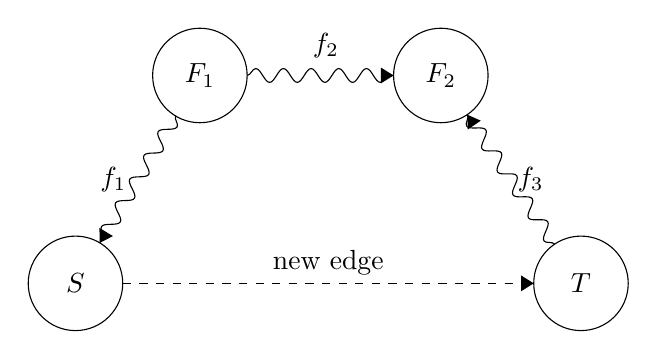
\begin{tikzpicture}[scale=0.2]
\tikzstyle{every node}+=[inner sep=0pt]
\draw [black] (18.1,-36.1) circle (3);
\draw (18.1,-36.1) node {$S$};
\draw [black] (50.2,-36.1) circle (3);
\draw (50.2,-36.1) node {$T$};
\draw [black] (26,-22.9) circle (3);
\draw (26,-22.9) node {$F_1$};
\draw [black] (41.3,-22.9) circle (3);
\draw (41.3,-22.9) node {$F_2$};
\draw [dashed] (21.1,-36.1) -- (47.2,-36.1);
\fill [black] (47.2,-36.1) -- (46.4,-35.6) -- (46.4,-36.6);
\draw (34.15,-35.6) node [above] {new edge};
\draw [decoration=snake,decorate] (24.46,-25.47) -- (19.64,-33.53);
\draw (20.5,-29.5) node {$f_1$};
\fill [black] (19.64,-33.53) -- (20.48,-33.1) -- (19.62,-32.58);
\draw [decoration=snake,decorate] (29,-22.9) -- (38.3,-22.9);
\draw (34,-21) node {$f_2$};
\fill [black] (38.3,-22.9) -- (37.5,-22.4) -- (37.5,-23.4);
\draw [decoration=snake,decorate] (48.52,-33.61) -- (42.98,-25.39);
\draw (47,-29.5) node {$f_3$};
\fill [black] (42.98,-25.39) -- (43.01,-26.33) -- (43.84,-25.77);
\end{tikzpicture}
\end{center}
\caption{Two flip tolerant path.}
\label{figure_two_flip}
\end{figure}

The two flip tolerant path search returns the set of all paths between a given source and sink that have up to two flips (paths that omit one or more of the three phases are also accepted).

The \textit{path extraction algorithm} then transforms the output of the two flip path search to the verification set, $Q' \cup C'$.

\paragraph{Path extraction algorithm}
Given a set of two flip tolerant paths from the new edge source to sink, the algorithm outputs a set of pairs to verify.

Let the new edge added to the diagram be $(S, T)$ and the input set of paths, $P$.
The algorithm processes every two flip tolerant path $p$ in $P$ case-wise to obtain pairs to add to the output set.
In the case where p has two flips, $t_1(p) \circ (S, T) \circ t_3(p)$ and $t_2(p)$ form a parallel pair.
When p has only the first flip (which is to say, the third phase of the path is missing), the parallel paths are $t_1(p) \circ (S, T)$ and $t_2(p)$.
Similarly when only the second flipping point is present (so that there is no first phase), then the parallel pair is  $(S, T) \circ t_3(p)$ and $t_2(p)$.
Finally when no flipping points are present, there are two possibilities.
Either $p$ is a path from $S$ to $T$, in which case the parallel paths are simply the edge $(S, T)$ and $p$, or $p$ is a path from $T$ to $S$.
In this case, we have found a cycle, $p \circ (S,T)$, to be paired with the identity function.
Like with the na\"{i}ve algorithm, for every node $v$ in the cycle, we add the pair $(v \rightarrow v, 1)$, where $v \rightarrow v$ is the cycle $p \circ (S,T)$ written to start and end at $v$.

\begin{theorem}
    Perform the two-flip tolerant path search from the source to sink node of the edge that is to be added followed, and on the output, apply the path extraction algorithm. 
    The result is the set $O = Q'\cup C'$ of new parallel pairs with exactly one path passing through the new edge and neither paths containing any cycles, and the set of simple cycles passing through the new edge.
\end{theorem}

\begin{proof}
    Every element in the output of the path extraction algorithm was by construction an element of $O$.

    It is also clear that every cycle in $C'$ can be expressed as $(S, T) \circ p$, and corresponds to the input two flip tolerant path p.
    
    It remains to show that every new parallel pair $p$ in $Q'$ corresponds to a two flip tolerant path.
    Let $\partial(p)^+ = F_1$ and $\partial(p)^- = F_2$. 
    Only one path passes through $(S, T)$. Let it be called $p_1$, and the other path, $p_2$.
    The two flip tolerant path from $S$ to $T$ can be constructed as follows: phase 1 is the segment of $p_1$ from $F_1$ to $S$, phase 2 is $p_2$, and phase 3 is the segment of $p_1$ from T to $F_2$.
    Effectively, $F_1$ corresponds to the first flipping point, and $F_2$, to the second.
    It is possible that some of $F_1, F_2, S$ and $T$ coincide (e.g., p starts at S --- $F_1 = S$), in which case the corresponding segments between the coinciding nodes can be considered the identity; the resultant path simply has fewer than two flips.        
\end{proof}

\paragraph{Analysis}
An upper bound on the number of pairs that this algorithm return is $O(|V|^{2} 2^{|V|})$, since two flip tolerant paths are an ordering on nodes, each node appearing at most once, followed by a selection of the flip points.
In practice, the algorithm significantly outperforms the Na\"{i}ve batch baseline because it looks only at parallel pairs that involve the new edge, usually a small subset of all parallel pairs.
Heuristic results are presented in the Section ~\ref{sec:evaluation}.

\subsection{Optimal batch solution}
Murota's main result ~\cite{commutative} is a solution to a batch version of \textsc{verification set}; given an acyclic diagram, it returns the minimal set of equality checks that would succeed if and only if the diagram commutes.
The paper describes an algorithm to find the ($|V|^2|E|$ bounded) minimal set of pairs that needs to be checked.

% A diagram's structure can result in some redundancy, in the sense that equivalence of a subset of pairs can imply the equivalence of path pairs that aren't in the subset.
% For example, in Figure ~\ref{figure_redundancies}, verifying $p_1$ and $p_2$ implies that the paths in $p_3$ are equal too.

% \begin{figure}
    
% \begin{center}
% \begin{tikzpicture}[scale=0.2]
% \tikzstyle{every node}+=[inner sep=0pt]
% \draw [black] (12,-15.8) circle (3);
% \draw [black] (30.5,-30.5) circle (3);
% \draw [black] (46.4,-15.8) circle (3);
% \draw [black] (29.9,-15.8) circle (3);
% \draw [black] (15,-15.8) -- (26.9,-15.8);
% \fill [black] (26.9,-15.8) -- (26.1,-15.3) -- (26.1,-16.3);
% \draw (20.95,-16.3) node [below] {$f_1$};
% \draw [black] (14.35,-17.67) -- (28.15,-28.63);
% \fill [black] (28.15,-28.63) -- (27.84,-27.74) -- (27.21,-28.53);
% \draw (19.94,-23.64) node [below] {$g_1$};
% \draw [black] (29.063,-27.873) arc (-157.62406:-197.70132:13.638);
% \fill [black] (29.06,-27.87) -- (29.22,-26.94) -- (28.3,-27.32);
% \draw (27.49,-23.25) node [left] {$f_2$};
% \draw [black] (31.53,-18.309) arc (25.84176:-21.16715:11.992);
% \fill [black] (31.53,-18.31) -- (31.43,-19.25) -- (32.33,-18.81);
% \draw (33.28,-23.03) node [right] {$j_1$};
% \draw [black] (32.9,-15.8) -- (43.4,-15.8);
% \fill [black] (43.4,-15.8) -- (42.6,-15.3) -- (42.6,-16.3);
% \draw (38.15,-16.3) node [below] {$j_2$};
% \draw [black] (32.7,-28.46) -- (44.2,-17.84);
% \fill [black] (44.2,-17.84) -- (43.27,-18.01) -- (43.95,-18.75);
% \draw (39.77,-23.64) node [below] {$h_1$};
% \end{tikzpicture}

% $p_1$=($f_1;f_2$, $g_1$)\\
% $p_2$=($j_1;j_2$, $h_1$)\\
% $p_3$=($g_1;h_1$, $f_1;j_2$)
% \end{center}
% \caption{Path checking redundancies: verifying $p_1$ and $p_2$ implies that the paths in $p_3$ are equal.}
% \label{figure_redundancies}
% \end{figure}

The approach in this algorithm, at a high level, is to define a function that takes in a subset of pairs and returns the subset of pairs whose equivalence is implied by the equivalence of the pairs in the input set.
Then the algorithm greedily eliminates redundancies until a minimal set is reached.

A bilinking is defined to be a parallel pair that is disjoint but for their terminal nodes. The set of all bilinkings is $R_0$.
In an acyclic diagram, if all bilinkings are equal, all parallel pairs must also be equal since they any given pair can be expressed as a composition of bilinkings.

Define $r_1>r_2$ for bilinkings $r_1$ = $\{p_1,q_1\}$, $r_2$= $\{p_2, q_2)$ $\in$ $R_0$, if there exists a path $p$ such that $\partial(p) = \partial(r_1)$ and $p$ contains $p_2$.
Define $\langle\rangle$ as:
$\langle r \rangle = \{ s\in R_0| r>s\}$.

For bilinking $s$, let $F(s)$ be the vector in $\text{GF}(2)^{|E|}$ representing the edges present in s (the $n^{\text{th}}$ dimension of $F(s)$ is 1 if the corresponding edge is in $s$, and 0 otherwise).
\xxx[AK]{GF(2) or $\mathbb{F}_2$ is standard notation for the Galois field of two elements. Do I need to write more about it here?}
Let this function be extended to sets, so that for some set of bilinkings $S, F(S) = \{ F(s) | s\in S \}$. A notion of linear independence in this vector field exists.

For a set of bilinkings $R$, the closure function $cl$ is defined as:
$cl(R) = \{ s\in R_0| s$ is linearly {dependent on $F(R) \}$.

The closure function on $R$ basically captures all the pairs that can be made by made by composing or ``gluing together'' the bilinkings in $R$. 

Using these two function we finally define the function $\sigma$ on a set of bilinkings R as
$\sigma(R) = \{s \in R_0 | s\in cl(R\cap \langle s \rangle) \}$.
This is the function used to capture all the pairs whose equivalence is implied by the equivalence of pairs in $R$.

$\sigma$ is used to iteratively check if a given pair is redundant.
Bilinkings are eliminated until a minimum ``spanning'' subset is reached.

Roughly, the algorithm proceeds by first efficiently finding a \textit{spanning} set of bilinkings (a subset whose verification implies the verification of all bilinkings in the graph).
It does this by, starting at every node, finding the reachable subsection of the graph, and a spanning tree for the subsection.
From each edges in the reachable section that is not a part of the tree, it generates a bilinking using the edge and a path in the tree that is parallel to the edge (~\ref{algo_spanning_set}).

\xxx[dg]{Probably put this in the appendix}
\begin{algorithm}
\label{alg_spanning_set}
\DontPrintSemicolon
\KwResult{Find a spanning set Rs = [$r_1$, ... ,$r_k$].}

Graph existingGraph\;
$R_s$ $\gets$ \{\}\;
\ForEach{node v in V}{
    S $\gets$ existingGraph.extractReachableSection(v)\;
    T $\gets$ createMinimumSpanningTree(S)\;
    excludedEdges = S.edges - T.edges\;
    \ForEach{edge e $\in$ excludedEdges}{
        firstPath = T.findPath(source: e.source, sink: e.sink)\;
        $R_s$.addElement(new Bilinking(firstPath, e)\;
    } 
}
\KwRet{$R_s$}\;

\caption{finding spanning set}\label{algo_spanning_set}
\end{algorithm}

With the spanning set thus initialized, it greedily tries to remove each pair from the spanning set if the set remains spanning even after removing the edge (~\ref{algo_minimal_spanning_set}).

\begin{algorithm}
\DontPrintSemicolon
\KwResult{Find a minimal spanning set R.}

\SetKwFunction{FSigma}{$\sigma$}
\SetKwProg{Fn}{Function}{:}{}
\Fn{\FSigma{inputSet S, codomain Rs}}{
    output $\gets$ \{\}\;
    \For{bilinking $\in$ Rs}{
        \tcc{Get fragments that could build up to the bilinking.}
        smallerPairs $\gets$ getSmallerPairs(bilinking)\;
        consideredPieces $\gets$ smallerPairs $\cap$ S \;
        \tcc{See if bilinking can be built from these pieces.}
        \If{linearlyDependent(consideredPieces, bilinking)}{
            output.add(bilinking)\;
        }
    }
    \KwRet{output}
}

R $\gets$ Rs\;
\For{i=1 to K}{
    \If{$r_i \in \sigma$(R-$r_i$)}{
       R $\gets$ R-$r_i$\;
    }
}
\KwRet{R}\;

\caption{Minimal spanning set}\label{algo_minimal_spanning_set}
\end{algorithm}

The proof of correctness can be found in Murota\cite{commutative}.
The number of checks returned by the algorithm is at worst $O(|V|^2|E|)$. The overall run time of an optimized implementation is $O(|V|^4|E|^2)$.

\section{Solving the online addition problem}

We present a polynomial time solution to the \textsc{verification set} problem.
Like with the baseline, we do not concern ourselves with parallel pairs where neither or both paths pass through the new edge.
The key observation that allows us to improve on the online baseline is that, for a given source and sink pair, only a single parallel pair needs to be verified. 
This is an implication of Theorem \ref{reductionRule}, expanded on later.
Theorem \ref{verifyingSet} shows that should our selected set of pairs along with cycles passing through the new edge be verified commutative, the entire diagram must commute. 
The approach is to identify a parallel pair with exactly one path through the edge for each (source, sink) pair (algorithm ~\ref{algo_online_polynomial}).

\begin{algorithm}
\DontPrintSemicolon
\KwData{existing graph, new edge.}
\KwResult{Set of parallel pairs to verify.}
\SetKwProg{try}{try}{:}{}
\SetKwProg{catch}{catch}{:}{end}
Graph existingGraph;
Edge newEdge;

parallelPairs $\gets$ \{\}\;
\For{S in existingGraph.Nodes}{
    \For{T in existingGraph}{
        \try{}{
            Path pathWithNewEdge $\gets$ FindPath(
                graph: existingGraph, 
                sourceNode: S,
                sinkNode: newEdge.Source()) +\;
            newEdge as Path +\;
            FindPath(
                graph: existingGraph, 
                sourceNode: newEdge.Sink(), 
                sinkNode: T)\;
            \If{S == T}{
                pathInOldGraph $\gets$ identity(S)\;
            }
            \Else(){
                Path pathInOldGraph $\gets$ FindPath(
                    graph: existingGraph, 
                    sourceNode: S, 
                    sinkNode: T)\;
            }
            parallelPairs.add((pathInOldGraph, pathWithNewEdge))\;
        }
        \catch{PathFindingFailedException}{
           \tcc{No comparable pairs from node S to node T that need to be checked}
           continue\;
        }
    }
}
\KwRet{parallelPairs}\;
\caption{Online polynomial time algorithm to find parallel pair set}
\label{algo_online_polynomial}
\end{algorithm}

The try block is executed at most $O(|V|^2)$ times, so that this is the bound on the number of pairs verified.

The bound is asymptotically tight. This can be seen in the case where the graph contains 2N nodes besides S and T. We consider N of the nodes to be in group 1, and the other N to be in group 2. Every node in group 1 has a forward node to every node in group 2, as well as to S. T has a forward edge to every node in group 2. In this diagram, on the addition of edge (S, T), $N^2$ paths need to be verified which is polynomial in 2N+2.

Also notice that if trying to optimize for path length (say, if composing functions is expensive) then "find any path" can be replaced with "find shortest path".

An efficient implementation of the algorithm can run in $O(|V|^2(|V|+|E|))$ time, space complexity not exceeding the asymptotic $O(|V|^2)$ bound on the output.
In such an implementation, path finding from a given source node to all potential sink nodes could be done in a single $O(|V|+|E|)$ breadth first search.

\subsection{Optimization Step}

In the case where equality checks are very expensive, we begin by finding the minimal set of (source, sink) pairs such that checking for these pairs logically implies having checked the full diagram.

We observe that there are some redundancies in the diagram.

Consider the situation in Figure ~\ref{figure_reduction_rule}.

\begin{figure}
\begin{center}
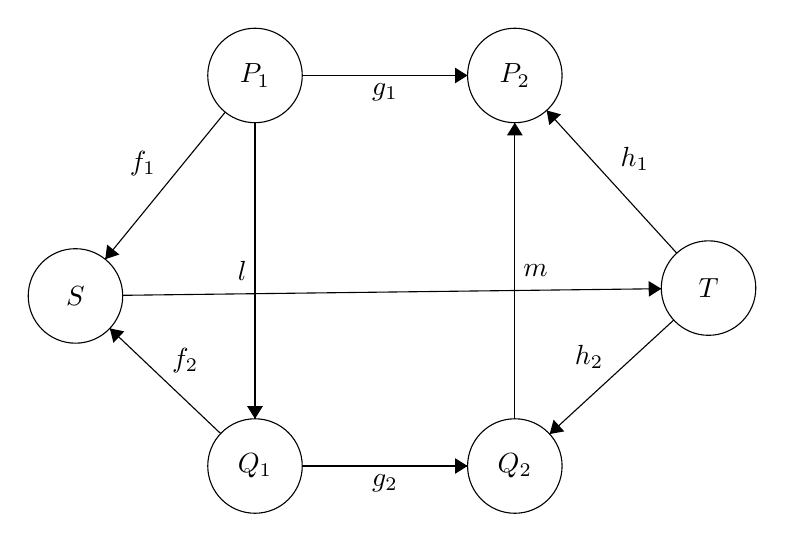
\begin{tikzpicture}[scale=0.2]
\tikzstyle{every node}+=[inner sep=0pt]
\draw [black] (16.6,-34.1) circle (3);
\draw (16.6,-34.1) node {$S$};
\draw [black] (56.8,-33.6) circle (3);
\draw (56.8,-33.6) node {$T$};
\draw [black] (28,-20.1) circle (3);
\draw (28,-20.1) node {$P_1$};
\draw [black] (44.5,-20.1) circle (3);
\draw (44.5,-20.1) node {$P_2$};
\draw [black] (28,-44.9) circle (3);
\draw (28,-44.9) node {$Q_1$};
\draw [black] (44.5,-44.9) circle (3);
\draw (44.5,-44.9) node {$Q_2$};
\draw [black] (31,-20.1) -- (41.5,-20.1);
\fill [black] (41.5,-20.1) -- (40.7,-19.6) -- (40.7,-20.6);
\draw (36.25,-20.6) node [below] {$g_1$};
\draw [black] (26.11,-22.43) -- (18.49,-31.77);
\fill [black] (18.49,-31.77) -- (19.39,-31.47) -- (18.61,-30.84);
\draw (21.74,-25.67) node [left] {$f_1$};
\draw [black] (25.82,-42.84) -- (18.78,-36.16);
\fill [black] (18.78,-36.16) -- (19.01,-37.08) -- (19.7,-36.35);
\draw (23.57,-39.02) node [above] {$f_2$};
\draw [black] (31,-44.9) -- (41.5,-44.9);
\fill [black] (41.5,-44.9) -- (40.7,-44.4) -- (40.7,-45.4);
\draw (36.25,-45.4) node [below] {$g_2$};
\draw [black] (54.59,-35.63) -- (46.71,-42.87);
\fill [black] (46.71,-42.87) -- (47.64,-42.7) -- (46.96,-41.96);
\draw (49.21,-38.76) node [above] {$h_2$};
\draw [black] (54.78,-31.38) -- (46.52,-22.32);
\fill [black] (46.52,-22.32) -- (46.69,-23.25) -- (47.43,-22.57);
\draw (51.19,-25.39) node [right] {$h_1$};
\draw [black] (28,-23.1) -- (28,-41.9);
\fill [black] (28,-41.9) -- (28.5,-41.1) -- (27.5,-41.1);
\draw (27.5,-32.5) node [left] {$l$};
\draw [black] (19.6,-34.06) -- (53.8,-33.64);
\fill [black] (53.8,-33.64) -- (52.99,-33.15) -- (53.01,-34.15);
\draw [black] (44.5,-41.9) -- (44.5,-23.1);
\fill [black] (44.5,-23.1) -- (44,-23.9) -- (45,-23.9);
\draw (45,-32.5) node [right] {$m$};
\end{tikzpicture}
Each arrow represents a path, and (S,T) is the new edge being added.
\end{center}
\caption{Reduction rule.}
\label{figure_reduction_rule}
\end{figure}

\begin{theorem}
\label{reductionRule}
If parallel paths $g_2 = f_2; (S,T); h_2$ then it must be that $g_1 = f_1; (S,T); h_1$.
\end{theorem} 
% monomorphisms
\begin{proof}
We use the fact that $f_1$=$l; f_2$ and $h_1$=$h_2; m$.
\[g_2 = f_2; (S,T); h_2 \Rightarrow l; g_2 = l; f_2; (S,T) ; h_2 \]
\[\Rightarrow l ; g_2 ; m = l ; f_2 ; (S,T) ; h_2 ; m \Rightarrow g_1 = f_1 ; (S,T) ; h_1\]
\end{proof}

The proof is not affected if any of these paths is the identity, eg. if $f_1$ is the identity and S and $P_1$ are actually the same node.

We conclude that verifying a comparable pair of paths with end points ($P_1$, $P_2$) implies the verification of all path pairs ($Q_1$, $Q_2$) such that $Q_1$ is a successor of $P_1$ and $P_2$ is a successor of $Q_2$. A successor S to node N is any node such that there exists a path from N to S. Nodes are also their own successors and predecessors.

Under the assumption that the only path operations allowed are composition and replacement of one path by a different, equal path, as would be true when edges are generic functions, and no other information is available, so that F is a semi-group, this "reduction" rule is also the only rule to reduce the set of path pairs to check by finding implications.

That is to say, if verifying a comparable pair of paths with end points ($P_1$, $P_2$) implies the verification of a pair with endpoints ($Q_1$, $Q_2$), then it must be that $Q_1$ is a successor of $P_1$ and $P_2$ is a successor of $Q_2$. %TODO proof required?

Using this information it is possible to choose a minimal subset of path pairs to verify, as in algorithm ~\ref{algo_online_minimal}.

We construct a graph with a node for each possible (source, sink) pair in the graph- each node then represents a possible choice for parallel pair endpoint pairs, and greedily search for the smallest set of nodes from which the entire graph would be reachable. The idea is to look for "roots" in the graph that have to be included in the ultimate verification set because they have no predecessor an cannot be verified "through" the verification of some other pair. Then all the successors whose verification is implied by the roots are eliminated.

\begin{algorithm}
\DontPrintSemicolon
\KwData{Existing graph, new edge.}
\KwResult{Set of parallel pairs to verify.}
Graph existingGraph\;
Edge (S, T)\;
        
predecessors $\gets$ S.predecessors(existingGraph)\;
successors $\gets$ T.successors(existingGraph)\;

Graph terminalPairGraph\;
\For{q $\in$ successors}{
    \For{p $\in$ predecessors}{
        terminalPairGraph.addNode(q, p)\;
        \For{qPred $\in$ q.predecessors(existingGraph)}{
            \For{pSucc $\in$ p.successors(existingGraph)}{
                terminalPairGraph.addEdge((qPred, pSucc))\;
            }
        }
    }
}

verificationSet $\gets$ \{\}\;
\While{len(terminalPairGraph.nodes) $>$ 0}{
    currentNode $\gets$ terminalPairGraph.nodes[0]\;
    visitedNodes $\gets$ \{\}\;
    \While{len(currentNode.parents()) $>$ 0}{
        visitedNodes.add(currentNode)\;
        currentNode $\gets$ currentNode.parents()[0]\;
        \If{currentNode $\in$ visitedNodes}{
            edges $\gets$ getAllEdges(visitedNodes, terminalPairGraph)\;
            terminalPairGraph.removeNodes(visitedNodes)\;
            terminalPairGraph.addNode(currentNode, edges)\; 
        }
    }
    verificationSet.add(currentNode)\;
    terminalPairGraph.removeNodes( currentNode.successors(terminalPairGraph))\;
}
\KwRet{verificationSet}\;
\caption{Minimal set finding algorithm}
\label{algo_online_minimal}
\end{algorithm}

The result of the algorithm cannot be further reduced.
Also, the verification of the parallel pairs returned in the algorithm implies that the output of the previous algorithm must commute, and transitively with Theorem ~\ref{verifyingSet} that the entire diagram must commute.

The run time of the first step is $O(|V|^4)$, and that of the second step is $O(|V|)$, so that the overall bound is $O(|V|^4)$.
Space complexity remains $O(|V|^2)$.

\subsection{Verification}
Ultimately verification is performed by calling an equality oracle (that is beyond the scope of this work) for every comparable pair returned by the previous stage, as in algorithm ~\ref{algo_verification}.

\begin{algorithm}
\DontPrintSemicolon
\For{(path1, path2) $\in$ parallelPairs}{
    \If{path1 $!$= path2}{
        \KwRet{False}\;
    }
}
\KwRet{True}\;
\caption{Verification algorithm}\label{algo_verification}
\end{algorithm}

\section{Applications}

\xxx[as]{Just a brief overview here to explain to the reader why these applications are important and appropriate (and what we hope to learn from the case studies).}

\subsection{Gator}
\label{sec:gator}

\xxx{Write the Gator section!}

\subsection{Currency Graph}
\label{sec:currency}

To demonstrate our algorithms applied to a real world situation, 
we found inconsistencies in a diagram of the exchange rate between currencies.
Consider a diagram with nodes as currencies and a directed edge being the
conversion rate from its source node's currency to its sink node's currency.
Since the transformation exchange rate of money from any given base currency to a target currency
can be expected to be the same regardless of which intermediate currency transformations
are used, this diagram should commute.

Using an API ~\footnote{https://exchangeratesapi.io}, we built the fully connected diagram of exchange rates between 32 currencies on a given day.
To ensure that it indeed commuted, we started with an empty diagram, and added in edges one by one.
Before the addition of each edge, we used the algorithms (~\ref{algo_online_polynomial} and ~\ref{algo_online_minimal}) to ensure the addition of a new edge did not introduce inconsistencies in the existing diagram.
If a new edge was, in fact, problematic, the algorithms returned an example inconsistent
pair that would arise from the addition of the edge.
The pair would consist of two currency transformation sequences with the 
same source currency and ultimate destination currency, but with different effective 
exchange rates values, as computed by taking the product of all the exchange rates
encountered through the chain.

We allowed an "error tolerance", so that differences reported would not be the trivial consequences of a floating point error.
However, this relaxation of the equality oracle into imprecision meant that the mathematical reasoning that allow the algorithms to remove redundant path checks no longer applied.
For instance, composing a new function with two approximately equal functions does not lead to equal results, so theorem ~\ref{reductionRule} fails with this approximate equality.
When the algorithms reported no inconsistencies, it was still possible that the graph possessed inconsistencies above the given threshold and did not commute.
Nonetheless, both algorithms were effective in catching inconsistencies. Algorithm ~\ref{algo_online_polynomial} started finding inconsistencies at error tolerances to the order of $10^{-3}$, and ~\ref{algo_online_minimal}, which makes more invalid redundant path check removals, at error tolerances to the order of $10^{-7}$.

Averaging over evaluation for the first 30 days of 2020, building and verifying a diagram to completion (inclusive of the time required by network calls) took 243$\pm$19 seconds using algorithm ~\ref{algo_online_minimal}, and in 133$\pm$13 seconds with algorithm ~\ref{algo_online_polynomial}. 

\section{Evaluation}
\label{sec:evaluation}
We compare performance of the following path checking algorithms: (1) Na\"{i}ve baseline (2) less Na\"{i}ve, two-flip baseline (3) batch baseline (4) algorithm ~\ref{algo_online_polynomial}, and (5) algorithm ~\ref{algo_online_minimal}.
The two aspects we look at are time for response and size of response set (smaller sets -- tighter output results -- would mean less calls to the oracle).
We use randomly generated graphs for benchmarking, and vary their size.
Given a graph and a new edge, we time how long it takes for an algorithm to return  the set of pairs that need to be verified.
All computation was performed on a Macbook Pro 2015, 2.9 GHz Dual-Core Intel Core i5.

The Na\"{i}ve baseline performs poorly, taking well over a thousand seconds for even small graphs of 10 nodes.
The batch algorithm brings timing down to seconds. Algorithm ~\ref{algo_online_polynomial} performs only slightly better.
Surprisingly, the optimal set algorithm cuts time cost by several orders of magnitude, and runs in milliseconds for small graphs.
All implementations are sensitive to density, performing better when density is very low or very high.

\subsection{Comparison of algorithm time cost}
The average time taken by each algorithm over the course of 10 runs over randomly generated graphs with 9 nodes and 32 edges is listed in Table ~\ref{tab:times}.

\begin{table}
\begin{tabular}{|c|c|}
    \hline
    Algorithm & average seconds of computation \\
    \hline
    Na\"{i}ve baseline & 0.77 \\
    Two Flip tolerant & 0.075 \\
    Batch algorithm & 7.55 \\
    ~\ref{algo_online_polynomial} & 0.0038 \\
    ~\ref{algo_online_minimal} & 0.00086 \\
    \hline
\end{tabular}
\caption{Computation time for 9 node graph of density 0.4, averaged over ten runs}
\label{tab:times} %TODO debug and fix label not working.
\end{table}
    
\subsection{Scaling of time with input size}

Algorithms scale as expected with time, as seen in Figure ~\ref{fig:timeVsSize}. 
Both ~\ref{algo_online_minimal} and ~\ref{algo_minimal_spanning_set} exhibit graphs that are polynomial in appearance.
The Na\"{i}ve baseline as well as the two flip tolerant baseline display quick growth.
The batch algorithm also grows fast, though not as much as the online checking baselines.

We define density to be the ratio of the number of edges in the graph to the total possible number of edges ($|V|^2$, where $|V|$ is the number of nodes).
Run time relates to the density of edges in the input graph.
The degree of the effect differs with the algorithms, as Figure ~\ref{fig:timeVsSize} shows.
Generally, denser graphs entail longer computation time.
For the batch algorithm we use lower densities since the input graph must be acyclic. This puts an upper bound on density that approaches 0.5 in large graphs.
% Our proposed algorithms, ~\ref{algo_minimal_spanning_set} and ~\ref{algo_online_polynomial} are less affected because they aggressively remove redundancies.

\begin{figure}
    % TODO format nicely.
    \begin{subfigure}{0.5\linewidth}
      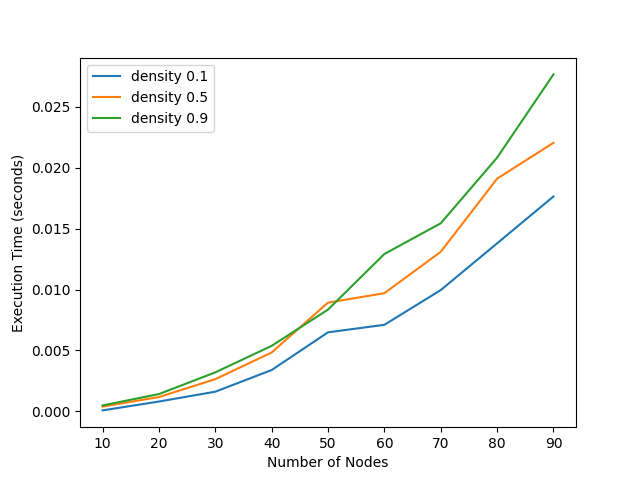
\includegraphics[width=.8\linewidth]{timeVsSize_10_OptimalSet.png}
      \caption{~\ref{algo_online_minimal}}
      \label{fig:sfigOptimalTvsS}
    \end{subfigure}

    \begin{subfigure}{0.5\linewidth}
      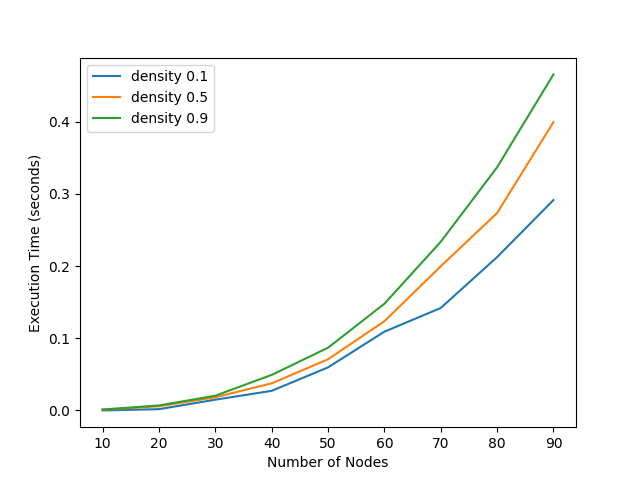
\includegraphics[width=.8\linewidth]{timeVsSize_10_Polynomial.png}
      \caption{~\ref{algo_online_polynomial}}
      \label{fig:sfigPolynomialTvsS}
    \end{subfigure}
    
    \begin{subfigure}{0.5\linewidth}
      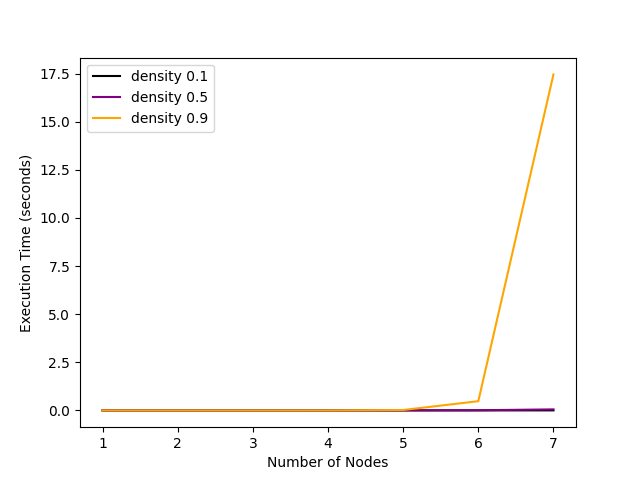
\includegraphics[width=.8\linewidth]{timeVsSize_10_NaiveChecker.png}
      \caption{Naive baseline}
      \label{fig:sfigNa\"{i}veTvsS}
    \end{subfigure}

    \begin{subfigure}{0.5\linewidth}
      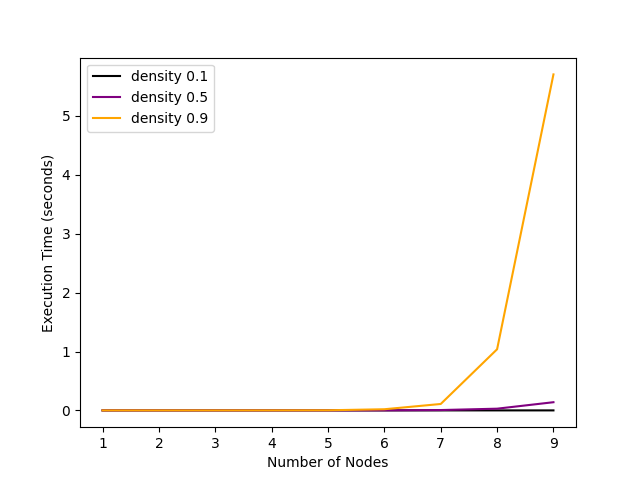
\includegraphics[width=.8\linewidth]{timeVsSize_10_TwoFlipPathChecker.png}
      \caption{Two flip tolerant baseline}
      \label{fig:sfigTwoFlipTvsS}
    \end{subfigure}

    \begin{subfigure}{0.5\linewidth}
      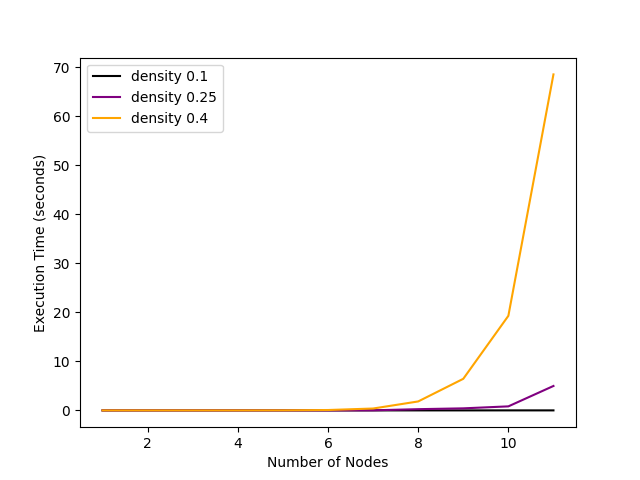
\includegraphics[width=.8\linewidth]{timeVsSize_10_BatchChecker.png}
      \caption{Batch algorithm baseline}
      \label{fig:sfigBatchTvsS}
    \end{subfigure}
    \caption{Plots of scaling of time with input size and density}
    \label{fig:timeVsSize}
\end{figure}

\subsection{Variance}
The periodic spikes in Figure ~\ref{fig:sfigOptimalTvsS} are striking. 
We plot the spread of results to understand what is happening.
We find ~\ref{algo_online_minimal} has outliers about two standard deviation above the mean responsible for the spikes in the average.
The outliers themselves follow a polynomial curve.
The plots in Figure ~\ref{fig:variance} depict the situation.
Grey points are the results of evaluation on individual points, and error bars show standard deviation. 
The black curve traces the mean.
No such effect is observed in ~\ref{algo_online_polynomial}.
\begin{figure}
    % TODO format nicely.
    \begin{subfigure}{0.5\linewidth}
      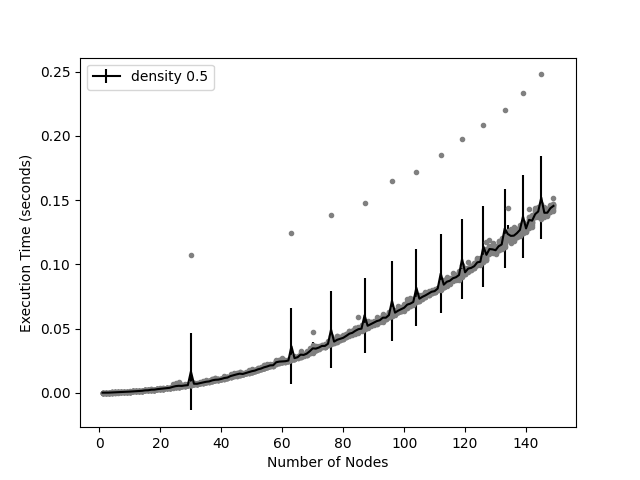
\includegraphics[width=.8\linewidth]{variance_10_OptimalSet.png}
      \caption{~\ref{algo_online_minimal}}
      \label{fig:sfigOptimalSpread}
    \end{subfigure}

    \begin{subfigure}{0.5\linewidth}
      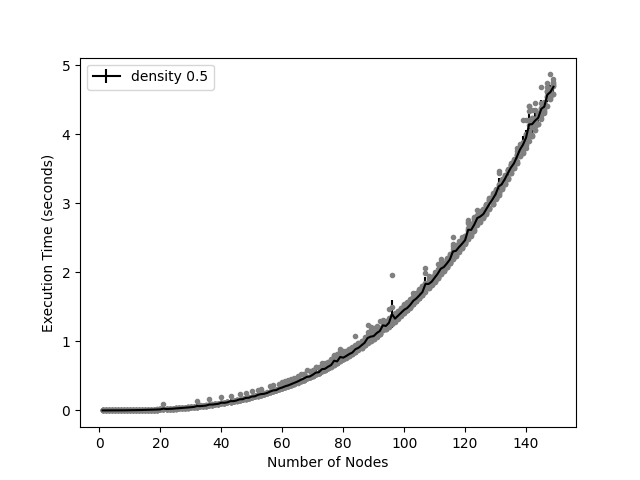
\includegraphics[width=.8\linewidth]{variance_10_Polynomial.png}
      \caption{~\ref{algo_online_polynomial}}
      \label{fig:sfigPolynomialSpread}
    \end{subfigure}
    
    \begin{subfigure}{0.5\linewidth}
      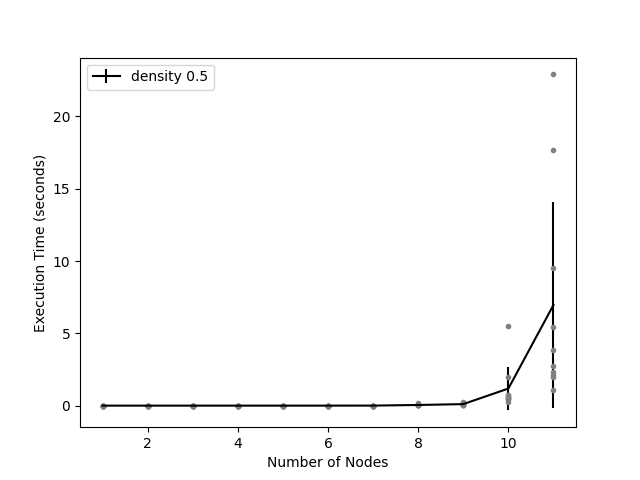
\includegraphics[width=.8\linewidth]{variance_10_TwoFlip.png}
      \caption{Two flip tolerant baseline}
      \label{fig:sfigTwoFlipSpread}
    \end{subfigure}

    \caption{Plots of spread of results}
    \label{fig:variance}
\end{figure}

\subsection{Size of Output}
Output size is a metric of interest, should the equality checking oracle be expensive.
Table ~\ref{tab:sizes}, summarizes the number of output pairs that the algorithms returned on average over 10 runs, for graphs with 9 nodes and 32 edges.
\begin{table}
\begin{tabular}{|c|c|}
    \hline
    Algorithm & average number of output pairs \\
    \hline
    Na\"{i}ve baseline & 39754.9 \\
    Two Flip tolerant & 748.9 \\
    Batch algorithm & 23 \\
    ~\ref{algo_online_polynomial} & 78.3 \\
    ~\ref{algo_online_minimal} & 1 \\
    \hline
\end{tabular}
\caption{Output size for 9 node graph of density 0.4, averaged over ten runs}
\label{tab:sizes}
\end{table}

\section{Appendix: Theorems and additional cases}

Consider all the cycles in the graph that pass through the new edge, unique to their terminal point.
Define a cycle-pair corresponding to cycle c to mean the pair of paths (c, identity on terminal node of c).
Let $C$ be the set of all cycle-pairs (unique to their terminal point) corresponding to cycles that pass through the new edge.

Let $V$, the set of pairs to verify, be $C \cup R_0$.

\begin{lemma}
\label{one_occurence_lemma}
A path that involves the new edge more than once is equal to a path without multiple occurrences of the edge, under the assumption that the pairs in C are verified.
\end{lemma}
\begin{proof}
Consider the part of the path between the first occurrence of the new edge and the second. This forms a cycle, which has a corresponding check in $C$ and must be verified to be equal to the identity.
This means that the loops containing the multiple occurrences of the new edge may be ignored and the path with a single occurrence of the new edge with the cycles removed is equal to this path.
\end{proof}

\begin{theorem}
\label{verifyingSet}
Verifying that all pairs in V commute implies that all pairs in $R_{all}$ commute.
\end{theorem}
\begin{proof}

Each pair in $R_{all}$ that is not in V would fall into one of these categories:

Case A: pairs that do not involve the new edge: By assumption that the original diagram commutes, these pairs must commute.

Case B: Cases where there is a different pair corresponding to this choice of (source, sink) in V already.
There are four paths to be considered, two from each pair. Those paths which do not include the new edge must already be equal by the assumption that the original diagram commutes.
Those paths which do include the new edge (S,T) can be reduced, by the case for multiple occurrences of a new edge, to a path with a single occurrence of the new edge as described in the preceding lemma \ref{one_occurence_lemma}. These new paths can be divided into three segments: the segment from the source to S, the new edge, and the segment from the last occurrence of T to the sink. The first segments of all paths are equal by assumption that the original diagram commutes. This is also true of the third segment of all the paths. The second segment consists of only the new edge and is the same for all paths. The composition of equal functions is equal, so all the paths passing through the new edge must be equal.
Therefore it is sufficient to check one path that passes through the new edge and one that doesn't. Such a pair belongs to V by construction.
\end{proof}

\section{Related Work}

\xxx{Absolutely nothing related to this was ever done.}

\section{Conclusion}

\xxx[as]{Write a conclusion.}

\bibliography{refs}
\bibliographystyle{plain}

\end{document}
